\chapter{Proposed approach}

In the previous chapter, a review of two splicing detection methods based on illuminant colors analysis has been presented. However, their effectiveness still needed to be improved for real forensic applications.

The approach proposed in this chapter has been developed to correct some drawbacks and mainly to achieve an improved accuracy over the two approaches presented in Chapter 1. 

\section{Overview}

Most of the times, the splicing detection process relies on the expert's experience and background knowledge. This process usually is time consuming and error prone once that image splicing is more and more sophisticated and an aural (e.g., visual) analysis may not be enough to detect forgeries.

This approach to detecting image splicing is developed aiming at minimizing the user interaction. 

The two methods, presented in the previous chapter \cite{carvalho2016illuminant} and \cite{fan2015image}, are now being used in synergy with each other, going to analyze each image at the same time looking for potential signs of forgery.

Starting from an image we want to analyze, the method will output a set of results.
\begin{itemize}
\item A classification \textbf{label} indicating whether an image is believed to be original or counterfeit.
\item A classification \textbf{score} indicating the confidence of the method output.
\item A \textbf{detection map} highlighting the detected spliced regions.
\end{itemize}

The proposed approach minimizes human interaction being fully automated. However, not both the modules can operate in any circumstance. The face splicing detection module will work only if there is a number of faces greater than or equal to two.

\section{Face splicing detection module}

\section{Region splicing detection module}

The second form of the algorithm is to implement the method proposed by Fan et al.\cite{fan2015image} with some changes in order to try to correct some of its major drawbacks presented in Section 1.7.

The splicing detection task performed by our approach consists in labelling a new image among two pre-defined classes (real and fake) and later pointing the face with higher probability to be the fake face. In this process, a classification model is created to indicate the class to which a new image belongs.

In summary, this module consists of the 6 main steps:

\begin{itemize}
\item \textbf{Image segementation}: relies on vertical and horizontal image segmentations. The outputs of this stage are two set of directional image bands. 
\item \textbf{Band illuminant estimation}: consists in estimating the illuminant color for each segmented band using 5 different GGE algorithms.
\item \textbf{Reference illuminant estimation}: consists in estimating the illuminant reference value for each direction.
\item \textbf{Feature vector evaluation}: relies on encoding the singular band illuminant information into a feature vector for further classification. The feature vector elements are the differences between the current illuminant color and the reference one.
\item \textbf{Band classification}: consists in labelling each image band into one of the know classes (real or fake) based on the previously learned classification model.
\item \textbf{Detection map}: using the classification output of the previous step, a detection map is build. The higher the value of this map, the higher the  resulting classification score for a single pixel.
\end{itemize}

\begin{figure}[h!]
  \centering
    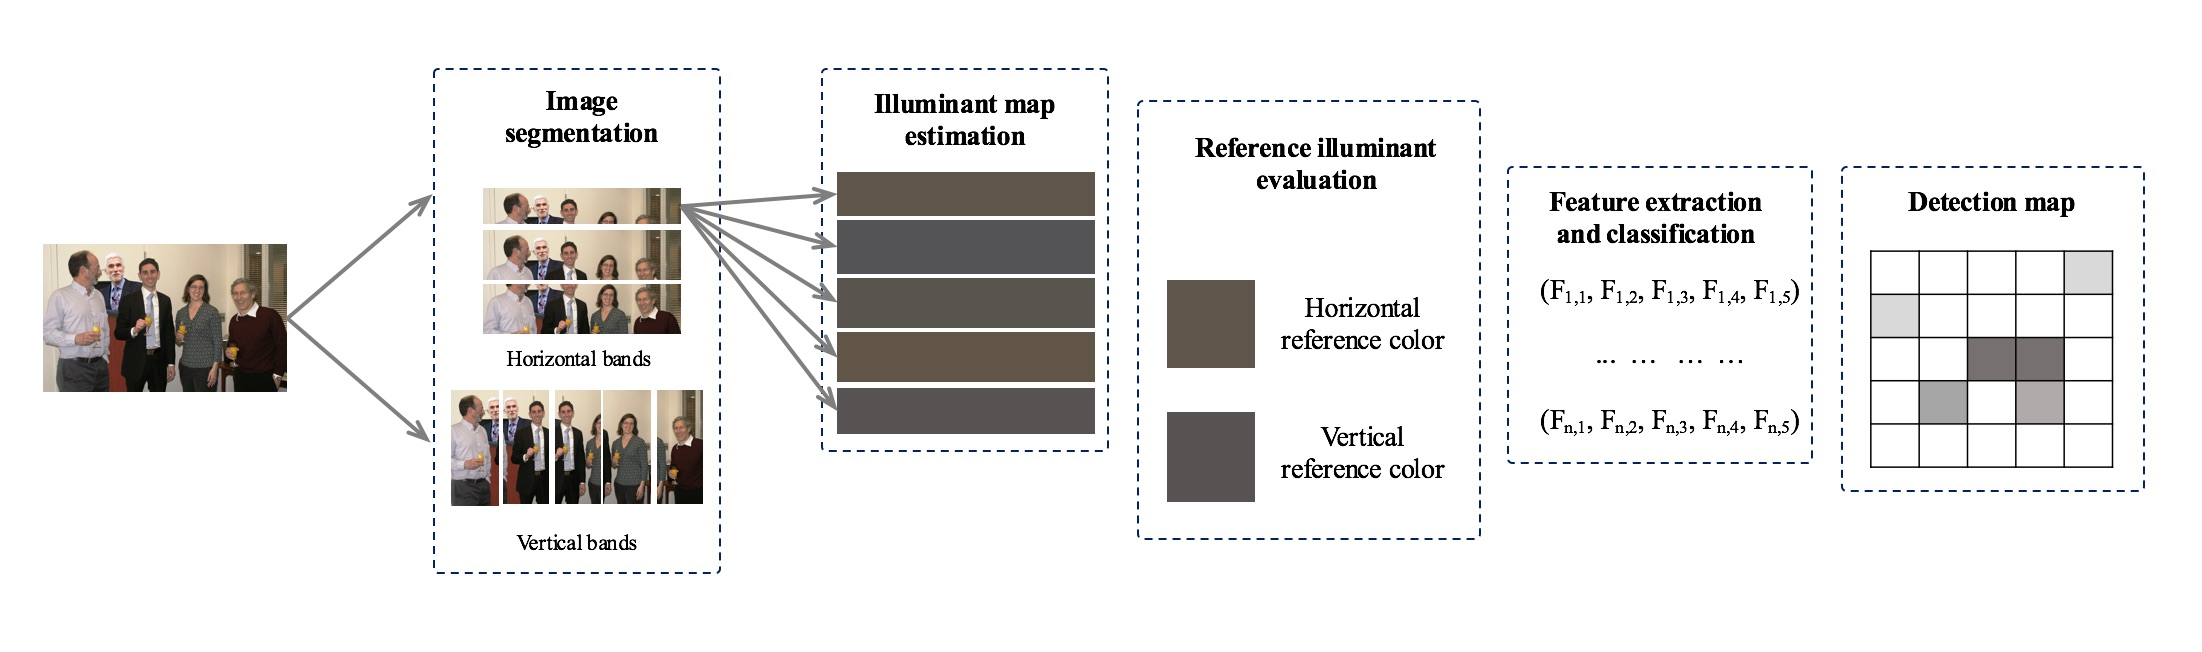
\includegraphics[width=1\textwidth]{pipeline_regions}
    \caption{Image regional splicing detection module pipeline}
    \label{fig:regionsmodulepipeline}
\end{figure}

The Fig \ref{fig:regionsmodulepipeline} summarize the module pipeline.

\subsection{Image segmentation}



\subsection{Band illuminant estimation}

\subsection{Reference illuminant estimation}

\subsection{Feature vector estimation}

\subsection{Band classification}

\subsection{Detection map}

